\documentclass[tikz, border=2pt]{standalone}
\usepackage{pgf,tikz}

\begin{document}
%Grafik:Zylinder
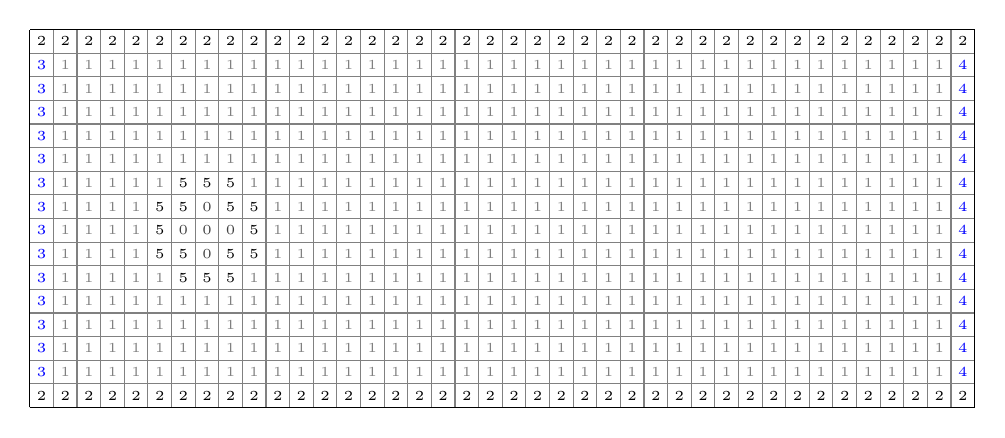
\begin{tikzpicture}[scale=1.5]
% lines
\draw[step=0.2, color=gray] (0,0) grid (8,3.2);
\draw [color=black] (0,0) -- (0,3.2);
\draw [color=black] (8,0) -- (8,3.2);
\draw [color=black] (0,0) -- (8,0);
\draw [color=black] (8,3.2) -- (0,3.2);
% cylinder, cross with zeros
\foreach \x in {1.3,1.7}
  \foreach \y in {1.5}
  \draw (\x,\y) node [anchor=center, color=black!75] {\tiny 0};
\foreach \x in {1.5}
  \foreach \y in {1.3,1.5,1.7}
  \draw (\x,\y) node [anchor=center, color=black!75] {\tiny 0};
% cylinder, left and right fives
\foreach \x in {1.1,1.9}
  \foreach \y in {1.3,1.5,1.7}
  \draw (\x,\y) node [anchor=center, color=black] {\tiny 5};
% cylinder, upper and lower fives
\foreach \x in {1.3,1.5,1.7}
  \foreach \y in {1.1,1.9}
  \draw (\x,\y) node [anchor=center, color=black] {\tiny 5};
% cylinder, fives in the corners
\foreach \x in {1.3,1.7}
  \foreach \y in {1.3,1.7}
  \draw (\x,\y) node [anchor=center, color=black] {\tiny 5};
% inflow left
\foreach \dy in {0.3,0.5,0.7,0.9}
  \foreach \y in {0,1,2}
  \draw (0.1,\y+\dy) node[anchor=center,color=blue] {\tiny 3};
  \draw (0.1,1.1) node[anchor=center,color=blue] {\tiny 3};
  \draw (0.1,2.1) node[anchor=center,color=blue] {\tiny 3};
% outflow right
\foreach \dy in {0.3,0.5,0.7,0.9}
  \foreach \y in {0,1,2}
  \draw (7.9,\y+\dy) node[anchor=center,color=blue] {\tiny 4};
\draw (7.9,1.1) node[anchor=center,color=blue] {\tiny 4};
\draw (7.9,2.1) node[anchor=center,color=blue] {\tiny 4};
% lower boundary
\foreach \x in {0,1,2,3,4,5,6,7}
  \foreach \dx in {0.1,0.3,0.5,0.7,0.9}
  \draw (\x+\dx,0.1) node[anchor=center] {\tiny 2};
% upper boundary
\foreach \x in {0,1,2,3,4,5,6,7}
  \foreach \dx in {0.1,0.3,0.5,0.7,0.9}
  \draw (\x+\dx,3.1) node[anchor=center] {\tiny 2};
% flow domain
\foreach \y in {.3,.5,.7,.9,1.1,1.3,1.5,1.7,1.9,2.1,2.3,2.5,2.7,2.9}
  \foreach \x in {0.2,2,3,4,5,6,7}
    \foreach \dx in {.1,.3,.5,.7}
      \draw (\x+\dx,\y) node[anchor=center,color=gray] {\tiny 1};
\foreach \y in {.3,.5,.7,.9,1.1,1.3,1.5,1.7,1.9,2.1,2.3,2.5,2.7,2.9}
  \foreach \x in {2.9,3.9,4.9,5.9,6.9}
      \draw (\x,\y) node[anchor=center,color=gray] {\tiny 1};
\foreach \x in {1.1,1.3,1.5,1.7,1.9}
  \foreach \y in {.3,.5,.7,.9,2.1,2.3,2.5,2.7,2.9}
    \draw (\x,\y) node[anchor=center,color=gray] {\tiny 1};
\draw (1.1,1.1) node[anchor=center,color=gray] {\tiny 1};
\draw (1.1,1.9) node[anchor=center,color=gray] {\tiny 1};
\draw (1.9,1.1) node[anchor=center,color=gray] {\tiny 1};
\draw (1.9,1.9) node[anchor=center,color=gray] {\tiny 1};
\end{tikzpicture}

\end{document}